\section{Monte Carlo Study}\label{sec:montecarlo}

% ---------------------------------------------------------------------------
\subsection{Design}\label{sec:mc_design}

We assess the finite-sample performance of the ZISAR estimator through a Monte~Carlo experiment that varies the sample size and the strength of spatial dependence.
The outcome $y_i$ is drawn from the ZISAR-NB specification defined in Section~\ref{sec:model_spec}: the latent predictor follows $\boldsymbol{\eta} = (\mathbf{I} - \rho\bW)^{-1}(\bX\bbeta + \bu)$ with $\bu \sim N(\mathbf{0},\sigma^2\mathbf{I})$, the count mean is $\mu_i = \exp(\eta_i)$, and the observation is $y_i = 0$ with probability $\pi_i$ (structural zero) or $y_i \sim \mathrm{NB}(\mu_i,\kappa)$ otherwise.
The spatial domain is a regular square lattice of side $n_{\text{side}} \in \{10, 15, 20\}$, yielding $n \in \{100, 225, 400\}$, and $\bW$ is the row-standardised queen-contiguity matrix.
The count covariates are $\bX = (\mathbf{1}_n, x_1, x_2)$ with $x_1,x_2 \overset{\mathrm{iid}}{\sim} N(0,1)$; the inflation covariates are $\bZ = (\mathbf{1}_n, z_1)$ with $z_1 \sim N(0,1)$.
The true parameter values are
\[
  \bbeta = (0.5,\; 0.8,\; -0.5)', \quad
  \bgamma = (-1.0,\; 0.4)', \quad
  \kappa = 2, \quad
  \sigma = 0.5,
\]
and the spatial parameter takes the values $\rho \in \{0, 0.15, 0.3, 0.45, 0.6\}$.
The data contain 43--52\% zeros, structural and sampling, fewer as $\rho$ grows, rates commonly observed in health-care utilisation data.
Each of the $5 \times 3 = 15$ scenarios is replicated $R = 1{,}000$ times.

In each replication we fit three specifications.
The ZINB \citep{cameron_trivedi2013}, estimated by \texttt{pscl::zeroinfl()} \citep{pscl}, ignores spatial dependence.
The SAR-NB is a negative binomial GLM that adds to the regressors the spatial lag of $\by$, instrumented by two-stage least squares with $\bH = [\bX, \bW\bX, \bW^2\bX]$, that is $\widehat{\bW\by} = \bH(\bH'\bH)^{-}\bH'\bW\by$; it ignores zero-inflation.
ZISAR is the proposed model in its restricted specification ($g_i \equiv 0$), estimated by \texttt{TMB} and the Laplace approximation.
For each estimator and for $\beta_1$, $\beta_2$, $\rho$ and $\kappa$ we compute the bias, $R^{-1}\sum_{r}(\hat{\theta}_r - \theta_0)$, and the root mean squared error (RMSE), $\bigl[R^{-1}\sum_{r}(\hat{\theta}_r - \theta_0)^2\bigr]^{1/2}$, over the replications in which the estimator converged, together with the median log-likelihood and the computing time.
For ZISAR we also exclude the fits in which $\hat\kappa$ exceeds~100, which in practice end at the upper bound $\kappa = 500$ of the optimisation box: in these fits the random effects absorb all the overdispersion and the count distribution is Poisson given~$\boldsymbol\eta$.
Their share, and the effect of keeping them, are reported below.

% ---------------------------------------------------------------------------
\subsection{Results}\label{sec:mc_results}

Figure~\ref{fig:mc} summarises the results; Tables~\ref{tab:mc_beta}--\ref{tab:mc_kappa} in Appendix~\ref{app:mc} report the bias, the RMSE and the median log-likelihood for $\rho \in \{0, 0.3, 0.6\}$.

\begin{figure}[htbp]
\centering
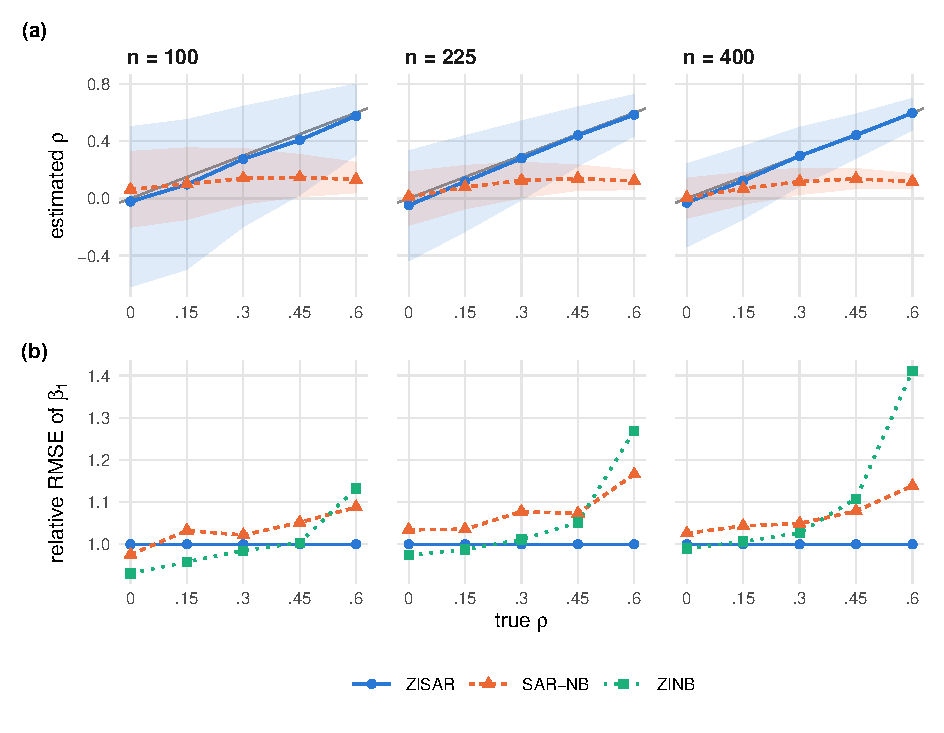
\includegraphics[width=\textwidth]{figures/mc_results.pdf}
\caption{Monte Carlo results, $R = 1{,}000$ replications per scenario. (a) Mean estimate of $\rho$ (lines) and 10th--90th percentiles across replications (bands) for the SAR-NB and ZISAR; the grey line marks the true value. The ZINB fixes $\rho = 0$. (b) RMSE of $\hat\beta_1$ relative to that of ZISAR in the same scenario: values above one favour ZISAR.}\label{fig:mc}
\end{figure}

ZISAR recovers the spatial parameter, whereas the SAR-NB does not (Figure~\ref{fig:mc}a).
Whatever the true value, the SAR-NB estimate stays below 0.15, so that its bias grows with $\rho$ and does not diminish with~$n$: at $\rho=0.6$ it is $-0.47$, $-0.48$ and $-0.48$ for $n = 100$, 225 and 400.
The two-stage procedure ignores the zero-inflated structure and the latent-field formulation, so that its instruments are misspecified.
The mean ZISAR estimate follows the true value at every sample size.
Its bias is small and negative in every scenario, never beyond $-0.052$, and at $\rho=0.6$ and $n=400$ it is $-0.002$, with an RMSE of~$0.087$.
The price is variance when the dependence is weak and the sample is small: at $\rho = 0$ the RMSE of ZISAR is 0.43 with $n=100$ and 0.23 with $n=400$, against 0.25 and 0.12 for the SAR-NB, whose estimate is held near zero.
The RMSE of ZISAR falls with both $n$ and $\rho$, and is below that of the SAR-NB from $\rho = 0.3$ with $n = 400$ and from $\rho = 0.45$ at every sample size.

Ignoring the spatial structure also affects the regression coefficients (Figure~\ref{fig:mc}b).
At $\rho = 0$ the three estimators have similar RMSE; with $n = 100$ ZISAR pays for the two parameters it estimates in vain, $\rho$ and~$\sigma$, with an RMSE of $\hat\beta_1$ 7\% above that of the ZINB, a gap that disappears at $n = 400$.
As $\rho$ grows the ZINB estimator of $\beta_1$ becomes biased upwards, by $0.056$ at $\rho = 0.6$ with $n = 100$ and by $0.066$ with $n = 400$, because the spatially correlated latent field is absorbed into the coefficients; its bias does not shrink with~$n$, whereas that of ZISAR stays below $0.02$ in absolute value in every scenario.
At $\rho = 0.6$ and $n = 400$ the RMSE of $\hat\beta_1$ is $0.079$ for ZISAR, $0.090$ for the SAR-NB and $0.111$ for the ZINB, 14\% and 41\% higher, and the RMSE of $\hat\beta_2$ is $0.072$, $0.084$ and $0.091$.
The efficiency gain of ZISAR grows with $\rho$ and, against the ZINB, with $n$, as the bias of the ZINB becomes the larger part of its RMSE.

The competitors also misattribute the overdispersion.
Because the ZINB estimate of $\kappa$ is occasionally very large, we compare medians.
Both competitors underestimate $\kappa$: the median bias is between $-1.40$ and $-1.52$ for the SAR-NB, which ignores the zero-inflation, and between $-0.70$ and $-1.10$ for the ZINB, growing with $\rho$ as the omitted spatial field adds extra-Poisson variation.
ZISAR has the smallest bias in every scenario, between $-0.34$ and $-0.56$.
The downward bias that remains reflects the trade-off between the random-effects variance $\sigma^2$ and the NB dispersion $\kappa^{-1}$, both of which generate overdispersion, and is accentuated by the exclusion of the fits at the upper bound of~$\kappa$.
ZISAR attains the highest median log-likelihood in every scenario (Table~\ref{tab:mc_kappa}).
Its gap over the ZINB is below one nat at $\rho=0$, where the two models coincide up to the variance component, and grows with $\rho$ and $n$, to 5, 8 and 16 nats at $\rho=0.6$ for $n=100$, $225$ and $400$.
The ZISAR log-likelihood is the Laplace-approximated marginal likelihood, including the Gaussian normalising constant $-\tfrac n2\log(2\pi)$, and the medians are computed over the retained fits, so that the comparison is indicative rather than a formal test, the competitors not being nested in ZISAR in the same way.

Finally, ZISAR converges in 97--100\% of the replications of every scenario.
The fits with $\hat\kappa$ at the upper bound are 12--17\% of the converged ones with $n = 100$, 7--9\% with $n = 225$ and 3--5\% with $n = 400$; keeping them changes the bias and the RMSE of $\hat\beta_1$ and $\hat\beta_2$ by at most $0.005$ and the RMSE of $\hat\rho$ by less than~$0.02$.
A fit, standard errors included, takes on average 0.1\,s with $n=100$, 0.25\,s with $n=225$ and 0.55\,s with $n=400$ on a single core, and the whole experiment, 45{,}000 fits, ran in nine minutes in parallel on a laptop.

% ---------------------------------------------------------------------------
\subsection{Power of tests for spatial dependence}\label{sec:mc_power}

In applied work, the presence of spatial dependence is often judged from Moran's $I$ \citep{moran1950,cliff_ord1973} computed on the residuals of an aspatial model.
In zero-inflated counts this test may lack power, because the spatial signal is diluted by the structural zeros and by negative binomial noise.
We compare it with the likelihood-based tests delivered by ZISAR in a second experiment.
The $n\in\{300, 900\}$ units have centroids drawn uniformly over a $2.5\times2$ box and $\bW$ is the row-standardised 6-nearest-neighbour matrix; four independent standard normal covariates enter the count process and one of them, together with a further independent covariate, enters the inflation process, with
$\bbeta = (1.2,\, 0.4,\, 0.3,\, 0.2,\, -0.15)'$, $\bgamma = (-1.5,\, 0.6,\, -0.4)'$, $\kappa = 2$ and $\sigma = 0.4$.
The covariates are spatially independent, a deliberately unfavourable setting for spatial methods: all the spatial structure in the outcome comes from the latent field.
For each $\rho\in\{0, 0.2, 0.35, 0.5, 0.7\}$ we draw 200 datasets and record how often each test rejects the absence of spatial dependence at the 5\% level (Table~\ref{tab:power_moran}).

\begin{table}[htbp]
\centering
\caption{Rejection rates at the 5\% level of tests for spatial dependence, 200 replications per cell. Zeros range from 35\% ($\rho=0$) to 21\% ($\rho=0.7$).}\label{tab:power_moran}
\small
\begin{tabular}{ll rrrrr}
\toprule
& & \multicolumn{5}{c}{true $\rho$} \\
\cmidrule(lr){3-7}
$n$ & Test & 0 & 0.2 & 0.35 & 0.5 & 0.7 \\
\midrule
\multirow{4}{*}{300}
 & Moran's $I$ on $\by$             & 0.060 & 0.135 & 0.285 & 0.560 & 0.925 \\
 & Moran's $I$ on ZINB residuals    & 0.045 & 0.085 & 0.215 & 0.445 & 0.915 \\
 & ZISAR Wald test on $\tilde\rho$  & 0.035 & 0.240 & 0.492 & 0.840 & 1.000 \\
 & ZISAR LR test of $\rho=0$        & 0.055 & 0.168 & 0.359 & 0.810 & 1.000 \\
\midrule
\multirow{4}{*}{900}
 & Moran's $I$ on $\by$             & 0.065 & 0.170 & 0.490 & 0.875 & 1.000 \\
 & Moran's $I$ on ZINB residuals    & 0.070 & 0.105 & 0.320 & 0.705 & 1.000 \\
 & ZISAR Wald test on $\tilde\rho$  & 0.061 & 0.327 & 0.863 & 1.000 & 1.000 \\
 & ZISAR LR test of $\rho=0$        & 0.086 & 0.276 & 0.817 & 1.000 & 1.000 \\
\bottomrule
\end{tabular}
\end{table}

Under the null all four tests have rejection rates close to the nominal 5\%, with the likelihood-ratio test somewhat liberal at $n=900$ (8.6\%).
Under the alternative the likelihood-based tests are uniformly more powerful.
The gap is largest at moderate dependence: at $\rho=0.35$ the Moran test on ZINB residuals detects the dependence in 22\% of samples with $n=300$ and 32\% with $n=900$, against 49\% and 86\% for the ZISAR Wald test.
The Moran test on residuals is also less powerful than the same test on the raw counts, because the aspatial model partly absorbs the spatial signal into its intercept and dispersion.
In zero-inflated count settings, a non-significant Moran statistic on residuals is therefore weak evidence of spatial independence, and inference on spatial dependence should rest on the structural parameter.
